\documentclass {CSEThesis}

% \usepackage[showframe , margin=1in , top = 0.5in]{geometry}
 
\usepackage[hidelinks]{hyperref}
\usepackage{amsmath}        % Extra math definitions
\usepackage{graphics}       % PostScript figures
\usepackage{setspace}       % 1.5 spacing
%\usepackage{psfig,epsfig}
\usepackage{multicol}
\usepackage{subfigure}
\usepackage{hyperref}
\usepackage{epsfig,color}
\usepackage{titlesec}
\usepackage{float}
\usepackage[T1]{fontenc}
\usepackage[utf8]{inputenc}

%% use this in your preamble
\usepackage{newunicodechar}
\newunicodechar{ff}{ff}
\newunicodechar{fi}{fi} 
\newunicodechar{fl}{fl}
\newunicodechar{ffi}{ffi}
\newunicodechar{ffl}{ffl}
%% end of common ligatures
% Custom packages
%\usepackage[first]{datestamp}   % Datestamp on first page of each chapter
\titleformat{\chapter}[display]   
{\normalfont\huge\bfseries}{\chaptertitlename\ \thechapter}{20pt}{\Huge}   
\titlespacing*{\chapter}{0pt}{-50pt}{40pt}

\usepackage{color}

\btptitle = {Railway Scheduling Using Reinforcement Learning} % { and } are needed around your name
\name = {Arpit Singh}          % and other feilds. don't remove.
\rollno = {111601031}
\email = {111601031@smail.iitpkd.ac.in}
\guide = {Dr. Chandra Shekar Lakshminarayanan}


\begin{document}
\let\cleardoublepage\clearpage
\begin{titlepage}
    \begin{center}
    \textheight 15.5in \textwidth 12.5in {\large\sf  \textbf{\the\btptitle}}\\[12ex]
    {\small{\textsl{ \textbf{A Project Report Submitted \\
    in Partial Fulfillment of the Requirements \\
    for the Degree of \\
    [3ex]\small \bf Bachelor of Technology}}}}\\
    [16ex] \emph{by}
    \\[2ex]
    {\sf \sf \textbf{\the\name}\\
                 (\the\rollno)}\\[1ex]
    \emph{under the guidance of}\\[2ex]
    {\sf \bf \the\guide} \\[7ex]
    
    \vspace{1.2in}
    
     \begin{figure}[!h]
    \centering
     
\includegraphics[width=0.15\textwidth]{IITPkdFullLogoColor}
     \end{figure}
    
    
    
    {\small\bf DEPARTMENT OF COMPUTER SCIENCE AND ENGINEERING}  \\[1ex]
    %{\small \bf{INDIAN INSTITUTE OF TECHNOLOGY PALAKKAD}}
    %\\[2ex]
    %
    %  {\color{red} \hrule height 0.5ex}
    % \vskip 1ex
    % May \the\year 
    \end{center}
    \end{titlepage}
    
\tableofcontents 
% \voffset=-0.8in
\addcontentsline{toc}{chapter}{List of Figures} 
\listoffigures 

\pagenumbering{arabic}
\def\headrulehook{\color{black}}      % Color the header rule

%========== Chapters
% \voffset = -0.2in;
% \typeout{}
% \chapter*{\centering Acknowledgements}
\quad Write acknowledgements, if your want to.


% \cleardoublepage
\typeout{}
\titleformat{\chapter}[display]{\normalfont\Large\bfseries}{}{11pt}{\Huge}
\chapter{Introduction}
\pagenumbering{arabic}\hspace{3mm}


The aim is to work on an algorithm for scheduling
bidirectional railway lines (both single- and multi-track) using a
framework of Reinforcement Learning. Given deterministic arrival/departure times for
 all the trains on the lines, their initial positions, 
 priority and halt times, traversal times, deciding on track allocations is a 
 job shop scheduling problem (NP Complete ). However, 
 due to the stochastic nature of the delays, 
 the track allocation decisions have to be made in a dynamic manner, 
 while minimising the total priority-weighted delay. 
 This makes the underlying problem one of decision making in of 
 stochastic event driven systems. 
The primary advantage of the proposed algorithm compared to
exact approaches is its scalability, and compared to heuristic
approaches is its solution quality.Improved solution quality is obtained because
of the inherent adaptability of reinforcement learning to specific
problem instances.

\vspace{\baselineskip}
This report is organised in 4 main chapters.Chapter 2 discusses the problem statement in length, 
Chapter 3 discusses the implementation of the simulator, Chapter 4 discusses the algorithm details and 
Chapter 5 discusses the experiments and results. Last chapter discusses about the future course of the project.

\cleardoublepage 
\typeout{}
% \newgeometry{margin = 1in , top = 0in}
% \voffset=-0.in
\chapter{Problem Statement}
% \titleformat{\section}{\large\bfseries}{\thesection}{1em}{\ }
\section{Indian Railways}
\pagenumbering{arabic}\hspace{3mm}

Let us first describe the nature of the railway system in this country. 
The Indian railway network is designed to consist of long ‘lines’ (a string of stations),
which connect with each other at ‘junction’ stations. Each station is composed 
of one or more parallel \textbf{tracks}, which may be associated with a fixed direction of 
traffic, or they could be bidirectional. Similarly, there are one or more tracks 
between each neighbouring pair of stations. These tracks are typically referred 
to as \textbf{sections}, in order to differentiate them from tracks actually at a station. 
The section tracks can also be unidirectional (fixed direction of train movement)
 or bidirectional. The Indian network typically consists of sections with one or two tracks. 
\\
\\
 \begin{figure}[H]
    \centering
    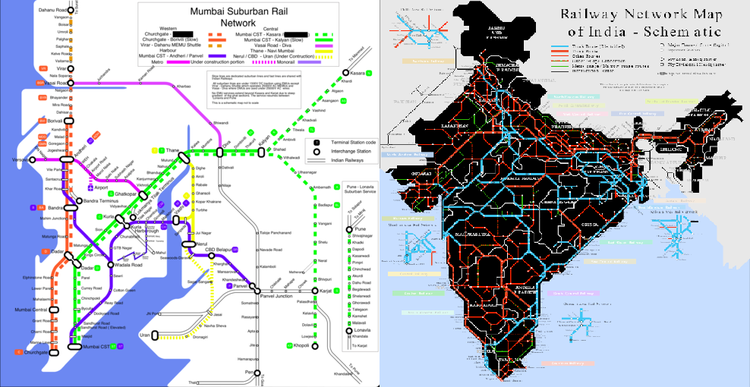
\includegraphics[width=0.8\textwidth]{Railways_pic}
    \caption{The line and junction topology of railway networks in India \cite{WEBSITE:1}. }
    \label{image-myimage}
\end{figure}

The approach we are focussing on now deals with linear railway 
networks with multiple parallel tracks, of the type shown in figure 2.2. This
restriction on topology is reasonable because rail networks are
designed in the form of multi-station linear arcs connected
at junction stations.

\begin{figure}[H]
    \centering
    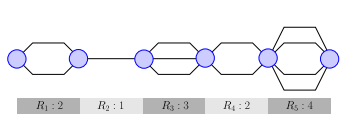
\includegraphics[width=0.4\textwidth]{report1}
    \caption{Linear Railway Lines \cite{ARTICLE:1}. }
    \label{image-myimage}
\end{figure}

\section{Railway Scheduling Problem}
\subsection{Scheduling}
A specific problem instance begins by defining the resources
on the railway line, as given by the number of stations, their
order, and the number of parallel tracks (both at each station
and between two neighbouring stations). Besides resource level information, 
train movements over the scheduling horizon must be described in one of two ways.
\begin{itemize}
    \item To define a reference timetable which gives the desired arrival
    and departure time of each train at each station.
    \item To provide the earliest movement times from their
    current locations (or origin stations), followed by the minimum
    running times (on track sections between stations) and halt
    times (at stations) up to the destinations.
\end{itemize}

\vspace{0.2cm}

Note that the running
and halt times can be completely heterogeneous: each train
may have a different running/halt time in each resource,
depending on the length of track, the type of halt, and the
type of locomotive.

\vspace{0.2cm}
Timetabling refers to an offline planning problem for a railway network.
\textbf{Given a set of trains and their origins and destinations (with or without a fixed route),
 the goal is to assign track resources for each train for a fixed time period, 
 such that they all complete their journeys without conflicts.}

 \vspace{0.2cm}
 Such a timetable may be infeasible if the desired arrival and
departure times violate the track usage rules defined earlier.
The task of the scheduling algorithm is to adjust the arrival
and departure times such that all rules are satisfied, while
minimizing an objective called priority-weighted delay. This schedule
is to be computed for all trains up to their destinations.

\vspace{0.2cm}
The railway problem has been shown in literature to be a \textbf{‘blocking’ version of the 
Job Shop Scheduling Problem (JSSP)}, where the job (train) must wait in the current resource 
(track) until the next resource is freed (there is no buffer for storing jobs between 
two resources). This version of the JSSP is also \textbf{NP complete}, with the result that 
exact solutions require an exponential amount of time for computation.
\vspace{1in}
\subsection{Rescheduling}

Another problem is that of rescheduling.
Rescheduling is the online counterpart of the timetabling problem , 
where the goal is to recover from a disruption to the timetable, 
caused by delays or faults. The mathematical differences are found in two aspects. 
\begin{itemize}
\item The goal is to return to the original timetable using built-in slack times, 
instead of defining the timetable itself. 
This implies that the objective function would focus on minimizing delays to 
trains with respect to the timetable, or the time required for deviations to the smoothed out. 
\item The online nature of the problem implies that there is very limited time 
available to compute solutions, and that sub-optimal but reasonably efficient 
solutions are acceptable. 
\end{itemize}

% \section{Time Table Scheduling problem}


\cleardoublepage 
\typeout{}
\chapter{Reinforcement Learning Approach}

\section{Brief Description}
Reinforcement learning works by learning to map the 
state of the system to the choice of available actions based on long-term reward 
(or penalty). In this report we will discuss review in brief the prior work \cite{ARTICLE:1} and then discuss the work that will be done as part of the project.  The key difference in both the
the approaches is:
\begin{itemize}
\item In the prior approach, we find state space with respect to train and it is the train that is making the 
decision (So we have the environment where each train is acting as the agent i.e. multiagent environment) 
\item In the proposed work, we have the central controller as the single agent and it is that
agent that is scheduling the trains.
\end{itemize}

\section {Prior Work}
\subsection{State Representation (Local state space)}

Here, we compute the state space as a function of \textbf{local neighborhood} of each
train.
A state vector is computed for each train every time a
decision about its next move is to be computed. Relative to
the direction of motion, we define resources as being behind
(in the direction opposite to the direction of motion) or in
front (in the direction of motion) of the train. A user-defined
finite number of resources $ l_b $ behind each train and $ l_f $ in
front of each train are used for defining the state vector. These
are referred to as local resources. Including a few resources
behind the train in the state definition ensures that overtaking
opportunities for fast-moving trains are not missed. The total
number of local resources is ($ l_b + 1 + l_f $). 
\vspace{0.2cm}
\begin{figure}[h]
    \centering
    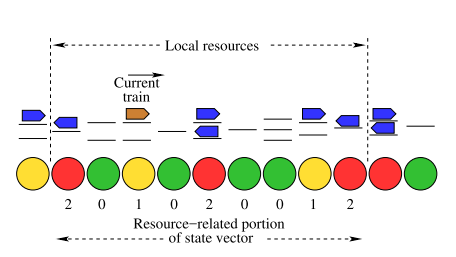
\includegraphics[width=0.8\textwidth]{report2}
    \caption{ Mapping train location and direction of movement to resource
    status, relative to the ‘current train’ \cite{ARTICLE:1}.  }
    \label{image-myimage}
\end{figure}


The entry in the state vector corresponding to each local
resource takes one of R integer values $ \{0, 1, 2,..., R-1\} $,
referred to as the status $S_r$ of resource $r$. Higher values
indicate higher congestion within the resource, and are driven
by the number of occupied tracks.
Let us define the number
of tracks in resource r to be equal to $N_r$, out of which $T_{r,c}$
tracks contain trains converging with (heading towards) the
current train, while $T_{r,d}$ tracks contain trains diverging from
(heading away from) the current train. Since at most one train
can occupy a given track, we note that $T_{r,c} + T_{r,d} < N_r$. The
mapping from track occupancy to resource status is,

$$ S_r = R - 1 - min(R - 1, \left \lceil{N_r - w_c T_{r,c} - w_d T_{r,d} }\right \rceil ).$$

Here, $0 \leq w_c$, $w_d \leq 1$ are weights that can de-emphasise
the effect of converging and diverging trains on the perceived
status of a resource.
\vspace{0.2cm}
We have one more entry in the state space for the priority of trains. If we assume that the model accommodates
up to $P$ priority levels, the size of the state space is equal to
\textbf { $ P \cdot R^{l_b+1+l_f} $}. Note that this value does not depend on the
scale of the problem instance, in terms of the number of trains,
the lengths of their journeys, and the number of resources.

\subsection {Action and Policy Definition}

In this approach, state space is computed for each train locally. 
The choice of actions in any given state is binary, with
0 representing a decision to move the current train to the next
resource on its journey, and 1 representing a decision to halt
in the current resource for a predefined time period (1 minute
in this paper). If the train is halted, the decision-making
procedure is repeated after the time period elapses.
 The policy that can be used to take the action is $ \epsilon$-greedy with the 
 value of $ \epsilon$-decresing over the training. It comprise of three steps 
 \begin{itemize}
\item Select the train on which to take the action.
\item Compute the state space for the train. 
\item Choose the action depending on the $\epsilon$-greedy policy. 
 \end{itemize}

\section{Proposed Approach}
\subsection {State Space Representation}
We are planning to use the whole network along with the positions of each train to take
as the state space. The key idea is to let the RL algorithm find which part of the state 
space is important to make decision. In the prior approach, we are kind of tuning how far the train can see and it's
action depends only on local neighborhood but in our work we are going to include everything in the state space.
Since, including everything can blow the size of the state space really quickly, so to tackle with this 
problem we can use function approximation methods (Deep Q-Learning) to learn the state space and then 
work on it.
\subsection{Action And Policy Definition}

In our proposed approach, we take the whole network topology and the position of the trains as the 
state space. So we have the central controller and that central controller will take the action for each train depending on 
state space that takes everything into account. 
At a particular time during the simulation, let's say we have n number of trains waiting for the 
action (ready to move or stop), then the controller have the action space of $2^n$ and it has to 
make decision for each of the trains (although in some order, as we are running the simulator and taking action 
for one train at a time).Size of the action space depends on the number of trains waiting for the 
action to be taken. Here again we can use the $\epsilon$-greedy policy for exploration in the initial phase
and then further exploitation.

\section {Objective Function}
A number of objective functions have been used in the
railway scheduling context, in order to achieve goals such
as delay reduction, passenger convenience, and timetable
robustness. One of the commonly used measures of
schedule quality is priority-weighted delay. A delay is
defined to be the non-negative difference between the time
of an event as computed by the algorithm, and the desired
time as specified by the timetable. The priority-weighted
average delay is the mean over all trains and all stations
of individual delays divided by train priorities. This quantity
is used as the objective function, but the algorithm can
accommodate other measures equally easily (for example,
a non-linear function of delays in order to increase fairness
of delay distribution).
$$ J = \frac{1}{N_{r,t}} \sum_{r,t} \frac{\delta_{r,t}}{P_t} $$
where $\delta_{r,t}$ is the delay for train t on departure from resource r,
$p_t$ is the priority of train t, and $N_{r,t}$ is the total number of
departures in the schedule. Note that this expression includes
all events for all trains, for their entire journey.

Prior work uses priority weighted delay as the objective function. In our proposed 
approach as well, we can shape the reward functions as to use the same
objective function.

\cleardoublepage 
\typeout{}
\chapter{Implementation}

As for now, we are focussing on how to implement the first approach 
and then move onto the second approach. The integrated reinforcement learning algorithm is driven
by a discrete event simulator. There are already some railway simulators like \textbf{OpenTrack} \cite{WEBSITE:2} and \textbf{RailML}\cite{WEBSITE:3} but they
would be useful for the final analysis of the results. Once we have the desired timetable then we can use these 
simulator softwares to determine the quality of solution. But for the implementation of the 
algorithm we have to implement the simulator on own.

\section {Railway simulator}
\subsection{Requirement}
The simulator is supposed to be robust enough that it can run both toy and real life 
examples. 
The simulator is suppose to run through several episodes during training and hence need 
to be efficient. At the
beginning of every episode, the initial locations of all the trains
are reset to their original values. It is assumed that trains that have not yet started, 
or have finished their journeys, do not
occupy any of the tracks. Following the train-to-resource mapping, 
the simulator creates a list of events for processing, one
corresponding to each train (whether already running or yet to
start its journey). Each event in the list contains the following
information: the time at which to process the event, the train to
which it corresponds, the resource where the train is currently
located, the last observed state-action pair for the train (empty
if the train is yet to start), and the direction of the train journey. 

At each step, the algorithm moves the simulation clock to
the earliest time stamp in the event list. If multiple events are to
be processed at the same time stamp, they are handled sequentially. We are for now 
not focussing on how to avoid deadlock, but instead if we get into deadlock, we will detect and give huge
negative reward and the RL algorithm is suppose to avoid deadlock on it's own.


\subsection{Implementation}
There are two components to railway simulator :
\begin{enumerate}
    \item Underlying Railway Network. 
    \item Trains and the simulation of there movements.
\end{enumerate}

For the implementation of the railway network we can use \textbf{NetworkX}\cite{WEBSITE:4} package of python.
\textbf{NetworkX is a Python package for the creation, manipulation,
and study of the structure, dynamics, and functions of complex networks.}
\vspace{1.5cm}

Once the network is ready we have to simulate movement of each train over the network. For 
that we can use \textbf{SimPy}\cite{WEBSITE:5} package of python. \textbf{SimPy is a process-based discrete-event simulation framework based on standard Python}.
In this we can model each train as the separate process and network as the resource. We can 
model the movement of trains using this package. We yield events when the train starts from some station and once 
the train reaches the next station, event is yielded and then we can process accordingly. So whole simulation is done 
by generating events at points where the algorithm is supposed to take action.


\cleardoublepage 
\typeout{}
\chapter{Conclusion and Future Work}

So far, focus is to fully understand the problem statement, what are the variations of the 
problem and then how RL algorithms can be used to solve this problem. The report discusses
two approach, to solve the problem. Currently the focus is to implement the prior approach and
see how good it is working, how good it is scaling to real life problem instances, how good it is 
performing compared to the present approaches and how to improve upon it. For the implementation of the 
algorithm, we need to implement the discrete railway simulator. For that, I have gone through the NetworkX and SimPy 
packages of standard python. The future plan is to complete the implementation of the simulator and then test 
our proposed method on the simulator.

Since we are tackling blocking version of the JSSP problem, so the approach that we will 
develop can be used to solve the JSSP problem with reasonable approximation. So the future plan is also 
to use the developed approaches on other similar problems as well.

\typeout{}

\bibliography{btp}
\bibliographystyle{IEEEtran}

\end{document}

